\documentclass[final,t]{beamer}\usepackage[]{graphicx}\usepackage[]{color}
%% maxwidth is the original width if it is less than linewidth
%% otherwise use linewidth (to make sure the graphics do not exceed the margin)
\makeatletter
\def\maxwidth{ %
  \ifdim\Gin@nat@width>\linewidth
    \linewidth
  \else
    \Gin@nat@width
  \fi
}
\makeatother

\definecolor{fgcolor}{rgb}{0.345, 0.345, 0.345}
\newcommand{\hlnum}[1]{\textcolor[rgb]{0.686,0.059,0.569}{#1}}%
\newcommand{\hlstr}[1]{\textcolor[rgb]{0.192,0.494,0.8}{#1}}%
\newcommand{\hlcom}[1]{\textcolor[rgb]{0.678,0.584,0.686}{\textit{#1}}}%
\newcommand{\hlopt}[1]{\textcolor[rgb]{0,0,0}{#1}}%
\newcommand{\hlstd}[1]{\textcolor[rgb]{0.345,0.345,0.345}{#1}}%
\newcommand{\hlkwa}[1]{\textcolor[rgb]{0.161,0.373,0.58}{\textbf{#1}}}%
\newcommand{\hlkwb}[1]{\textcolor[rgb]{0.69,0.353,0.396}{#1}}%
\newcommand{\hlkwc}[1]{\textcolor[rgb]{0.333,0.667,0.333}{#1}}%
\newcommand{\hlkwd}[1]{\textcolor[rgb]{0.737,0.353,0.396}{\textbf{#1}}}%

\usepackage{framed}
\makeatletter
\newenvironment{kframe}{%
 \def\at@end@of@kframe{}%
 \ifinner\ifhmode%
  \def\at@end@of@kframe{\end{minipage}}%
  \begin{minipage}{\columnwidth}%
 \fi\fi%
 \def\FrameCommand##1{\hskip\@totalleftmargin \hskip-\fboxsep
 \colorbox{shadecolor}{##1}\hskip-\fboxsep
     % There is no \\@totalrightmargin, so:
     \hskip-\linewidth \hskip-\@totalleftmargin \hskip\columnwidth}%
 \MakeFramed {\advance\hsize-\width
   \@totalleftmargin\z@ \linewidth\hsize
   \@setminipage}}%
 {\par\unskip\endMakeFramed%
 \at@end@of@kframe}
\makeatother

\definecolor{shadecolor}{rgb}{.97, .97, .97}
\definecolor{messagecolor}{rgb}{0, 0, 0}
\definecolor{warningcolor}{rgb}{1, 0, 1}
\definecolor{errorcolor}{rgb}{1, 0, 0}
\newenvironment{knitrout}{}{} % an empty environment to be redefined in TeX

\usepackage{alltt}




%% Examples:
%% http://www-i6.informatik.rwth-aachen.de/~dreuw/latexbeamerposter.php
\mode<presentation> {
  %% TODO(chogg): define my own theme
  %% (e.g. for big headlines using my own logos)
  \usetheme{I6pd2}
}
\usepackage[english]{babel}
\usepackage[latin1]{inputenc}
\usepackage{amsmath,amsthm,amssymb,latexsym}
\usepackage{pifont}
\newcommand{\cmark}{\ding{51}}%
\newcommand{\xmark}{\ding{55}}%
\usefonttheme[onlymath]{serif}
\boldmath
\usepackage[orientation=landscape,size=a0,scale=1.4,debug]{beamerposter}
\title[Smooth Animations]{\huge Smooth Animations to Visualize Gaussian Uncertainty}
\author{Charles~R.~Hogg~III}
\institute[Google]{Google, Inc.}
\date{July 16, 2014}
\IfFileExists{upquote.sty}{\usepackage{upquote}}{}
\begin{document}

\setlength{\leftmargini}{1.5em}

\begin{frame}[fragile]
  \vspace{-0.5em}
  \begin{columns}[T,onlytextwidth]

    % Left column.
    \begin{column}{.325\linewidth}

      \vbox to .698\textheight{%
      \begin{block}{Introduction}
        \vspace{-0.5em}
        \begin{itemize}
          \item \textbf{Goal:} Visualize uncertainty in \textit{curves and
            surfaces}
            \begin{itemize}
              \item Specifically: using \textbf{Gaussian processes}
                (see refresher at bottom)
            \end{itemize}
          \item \textbf{Approach:} animations
            \begin{itemize}
              \item Each frame shows one draw from posterior
              \item Consecutive frames show similar curves
                (i.e., \textit{continuous} animations)
              \item \textit{Reducible}:
                find \textbf{single ``Gaussian oscillator''};
                use copies as needed
            \end{itemize}
          \item \textbf{New Results:}
            \begin{itemize}
              \item \textbf{Smooth, keyframe-free} animations
              \item \textbf{New framework} for all future work in Gaussian
                animations
            \end{itemize}
        \end{itemize}
      \end{block}

      \vfill

      \begin{block}{Existing approach:
        interpolate between I.I.D. Gaussian draws}
        \vspace{-0.5em}
        Linear interpolation: \textbf{variance too small} between keyframes
\begin{knitrout}
\definecolor{shadecolor}{rgb}{0.969, 0.969, 0.969}\color{fgcolor}
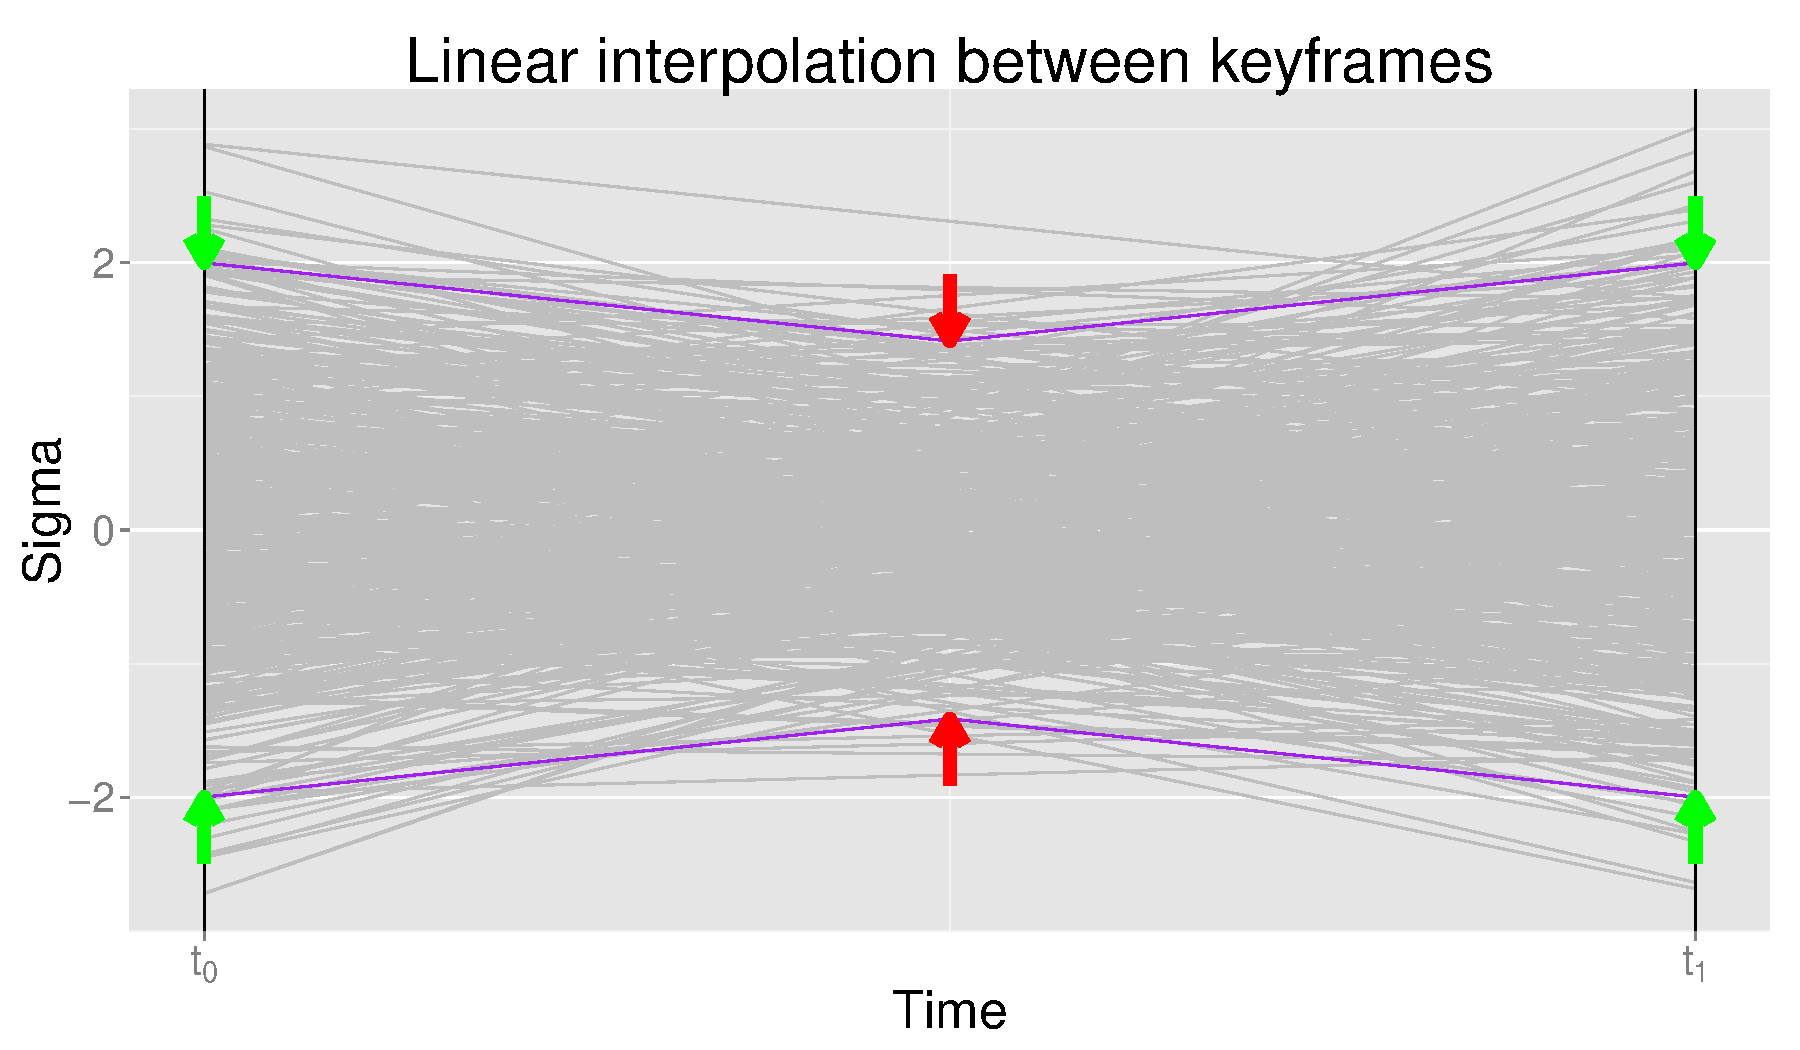
\includegraphics[width=\maxwidth]{figure/interpolation} 

\end{knitrout}

        \begin{itemize}
          \item Ehlschlaeger, Shortridge, Goodchild (\textbf{ESG})
            solved in 1997 (see right figure)
          \item Problem with \textit{both} approaches: keyframes are `special'
            \begin{itemize}
              \item Motion changes discontinuously
              \item Even at $\Delta t = 1$, correlation can be surprisingly high
                (up to 0.5)
            \end{itemize}
        \end{itemize}
      \end{block}

      \vfill

      \begin{block}{New approach: eliminate keyframes entirely}
        \vspace{-0.5em}
        \begin{itemize}
          \item Still use I.I.D. normals, $\{\epsilon_i\}$,
            but \textit{de-localize} rather than interpolate
        \end{itemize}
        \begin{equation*}
          f(t) = \frac{1}{\sqrt{N}} \sum_{i=1}^N
          \left[
            \epsilon_{2i-1}\sin\left(\frac{\pi i t}{N}\right) +
            \epsilon_{2i}  \cos\left(\frac{\pi i t}{N}\right)
          \right]
        \end{equation*}
        \begin{itemize}
          \item Correct statistical properties: 
            $\langle f(t) \rangle = 0$; \hspace{1em}
            $\langle f(t)^2 \rangle = 1$ \hspace{1em}
            $\forall t$
        \end{itemize}
      \end{block}

      }%
    \end{column}

    % Middle column.
    \begin{column}{.325\linewidth}

      \vbox to .698\textheight{%
      \begin{block}{Basis function view}
        \vspace{-0.8em}
        $$\textstyle f(t) = \sum\limits_{i=1}^N \epsilon_i b_i(t)$$
        \begin{table}
          \begin{tabular}{|l|c|c|c|}
            \hline
            Animation Method
            & \parbox[t][2.5em]{5em}{Statistically \\ Correct}
            & Stationary
            & Smooth \\
            \hline
\begin{knitrout}
\definecolor{shadecolor}{rgb}{0.969, 0.969, 0.969}\color{fgcolor}
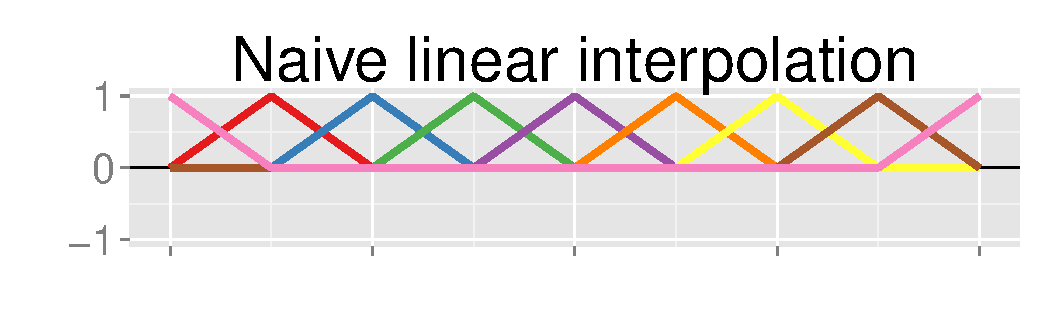
\includegraphics[width=\maxwidth]{figure/basis_linear} 

\end{knitrout}

            & {\Huge \color{red}{\xmark}} & {\Huge \color{red}{\xmark}} &
            {\Huge \color{red}{\xmark}} \\
            \hline
\begin{knitrout}
\definecolor{shadecolor}{rgb}{0.969, 0.969, 0.969}\color{fgcolor}
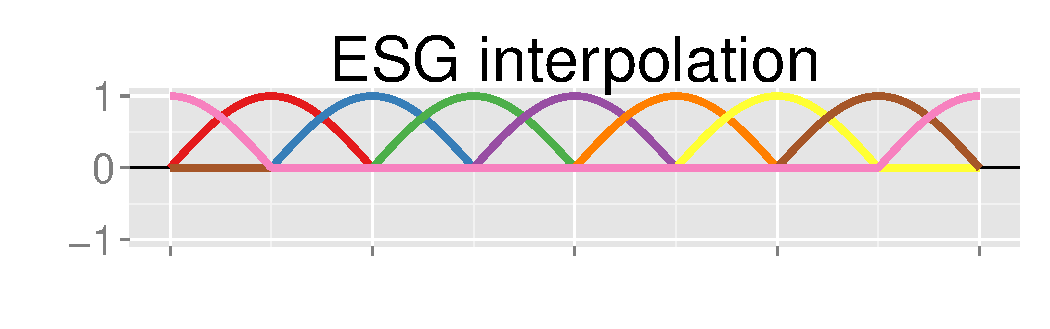
\includegraphics[width=\maxwidth]{figure/basis_esg} 

\end{knitrout}

            & {\Huge \color{green}{\cmark}} & {\Huge \color{red}{\xmark}} &
            {\Huge \color{red}{\xmark}} \\
            \hline
\begin{knitrout}
\definecolor{shadecolor}{rgb}{0.969, 0.969, 0.969}\color{fgcolor}
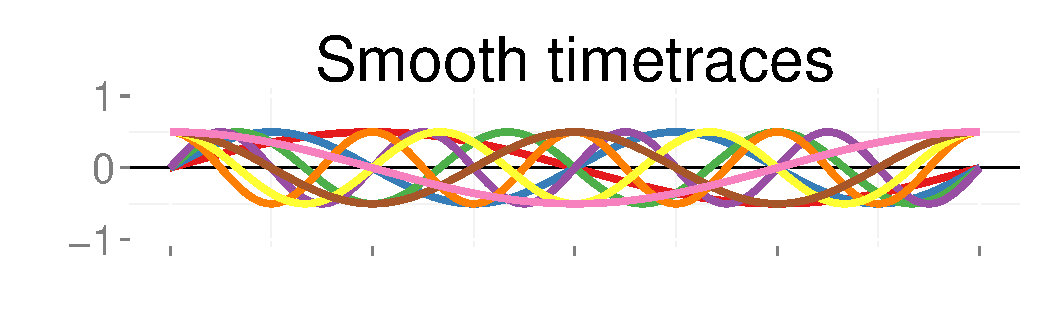
\includegraphics[width=\maxwidth]{figure/basis_smooth} 

\end{knitrout}

            & {\Huge \color{green}{\cmark}} & {\Huge \color{green}{\cmark}} &
            {\Huge \color{green}{\cmark}} \\
            \hline
          \end{tabular}
        \end{table}

      \end{block}

      \vfill

      \begin{block}{Physical motion: basic kinematics}
        {\small Check \textit{velocity} and \textit{acceleration} for a
        fuller picture of how these animations move:} \\
\begin{knitrout}
\definecolor{shadecolor}{rgb}{0.969, 0.969, 0.969}\color{fgcolor}
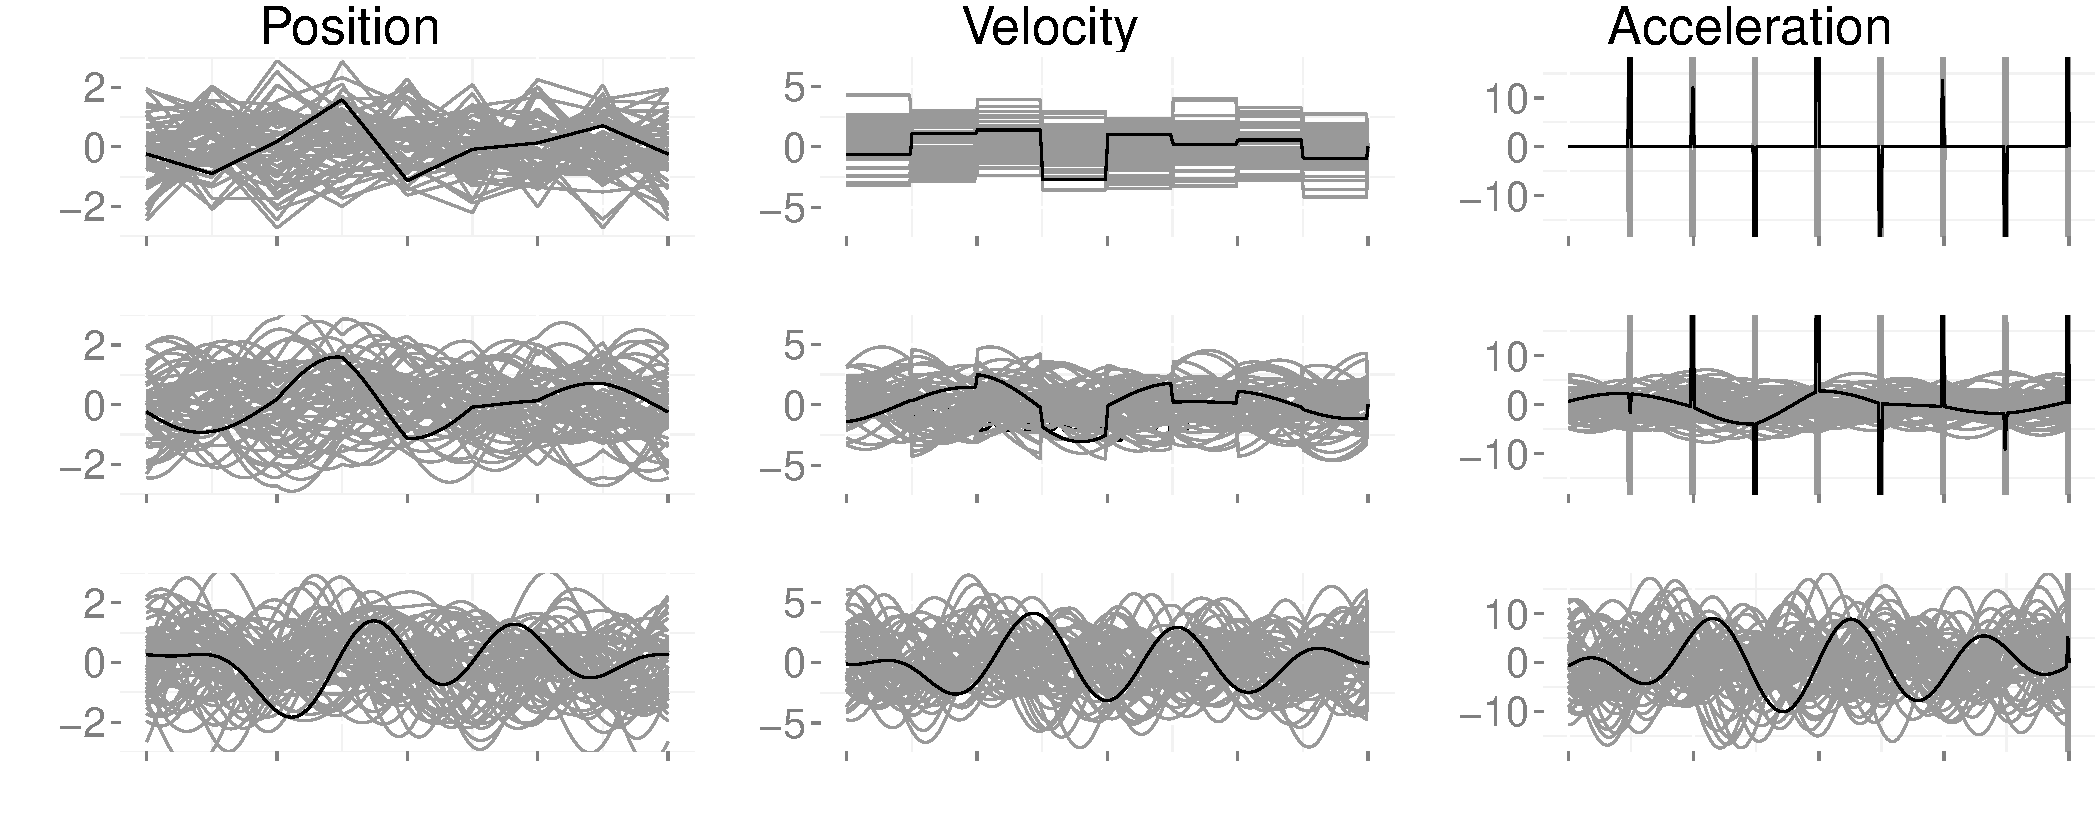
\includegraphics[width=\maxwidth]{figure/kinematics} 

\end{knitrout}

        Motion is \textit{not different} at the keyframes
        \textbf{because they do not exist.}
      \end{block}

      }%
    \end{column}

    % Right column.
    \begin{column}{.325\linewidth}

      \vbox to .698\textheight{%
      \begin{block}{The true nature of $f(t)$}
        \begin{itemize}
          \item Observations about $f(t)$:
            \begin{itemize}
              \item Infinite set of Gaussian random variables
              \item Indexed by continuous variable, $t$
              \item Well-defined covariance between every pair of points:
                \begin{equation*}
                  \langle f(t) f(t + \tau) \rangle = \frac{1}{N} \sum_{i=1}^{N}
                  \left[ 
                    \cos \left( \frac{\pi i \tau}{N} \right)
                  \right]
                \end{equation*}
            \end{itemize}
          \item \textbf{Implication:} $f(t)$ is
            \textit{itself a Gaussian process}
            (in the \textit{time} domain)
          \item \textbf{Benefit:} Gaussian animations
            \textit{revealed to belong to a \\ well-studied framework}
            \begin{itemize}
              \item Future animations can leverage existing Gaussian Process
                work
                \\ (e.g., try new covariance functions)
            \end{itemize}
        \end{itemize}
      \end{block}

      \vfill

      \begin{block}{\texttt{R} implementation}
\begin{knitrout}\tiny
\definecolor{shadecolor}{rgb}{0.969, 0.969, 0.969}\color{fgcolor}\begin{kframe}
\begin{alltt}
\hlcom{# Matrix to turn 2N random values into Gaussian oscillator.}
\hlstd{GaussianOscillatorMatrix} \hlkwb{<-} \hlkwa{function}\hlstd{(}\hlkwc{N}\hlstd{,} \hlkwc{t}\hlstd{) \{}
  \hlstd{(}\hlkwd{cbind}\hlstd{(}\hlkwd{outer}\hlstd{(t,} \hlnum{1}\hlopt{:}\hlstd{N,} \hlkwa{function}\hlstd{(}\hlkwc{x}\hlstd{,} \hlkwc{y}\hlstd{)} \hlkwd{cos}\hlstd{(pi} \hlopt{*} \hlstd{x} \hlopt{*} \hlstd{y} \hlopt{/} \hlstd{N)),}
         \hlkwd{outer}\hlstd{(t, N}\hlopt{:}\hlnum{1}\hlstd{,} \hlkwa{function}\hlstd{(}\hlkwc{x}\hlstd{,} \hlkwc{y}\hlstd{)} \hlkwd{sin}\hlstd{(pi} \hlopt{*} \hlstd{x} \hlopt{*} \hlstd{y} \hlopt{/} \hlstd{N)))}
   \hlopt{/} \hlkwd{sqrt}\hlstd{(N))}
\hlstd{\}}
\end{alltt}
\end{kframe}
\end{knitrout}

      \end{block}

      \vfill

      \begin{block}{Conclusions}
        \begin{itemize}
          \item First \textit{statistically correct} Gaussian animations with
            \textbf{smooth and \\ natural motion}
          \item Moving beyond interpolation: \textbf{keyframes entirely
            eliminated}
            
          \item \ \vspace{-1.2em} \\
            { \centering
              \textbf{Time-domain Gaussian Processes}
              \\ enable \textit{animated visualization} of 
              \\ \textbf{Space-domain Gaussian Processes}
              \begin{itemize}
                \item To eliminate keyframes,
                  use \textit{stationary} covariance function
              \end{itemize}
            }
        \end{itemize}
      \end{block}

      }%
    \end{column}

  \end{columns}

  \vspace{0.5em}
  \begin{beamercolorbox}[wd=0.9875\paperwidth]{sepline}
    \centering
    \rule{0pt}{3pt}
  \end{beamercolorbox}

  \begin{block}{Gaussian Processes refresher: Probabilities for Functions}
    \begin{columns}[T]
      \begin{column}{0.16\linewidth}
        \begin{itemize}
          \item Random curves and surfaces: \\
            \textit{infinitely many} random variables!
          \item \textbf{Gaussian Processes:} \\
            work with \textit{any \textbf{finite} subset}
            \begin{itemize}
              \item Assume \textit{joint Gaussian distribution}
            \end{itemize}
          \item Simple example: \\
            Start with 2 variables, \\
            work up from there...
        \end{itemize}
      \end{column}
      \begin{column}{0.12\linewidth}
\begin{knitrout}
\definecolor{shadecolor}{rgb}{0.969, 0.969, 0.969}\color{fgcolor}
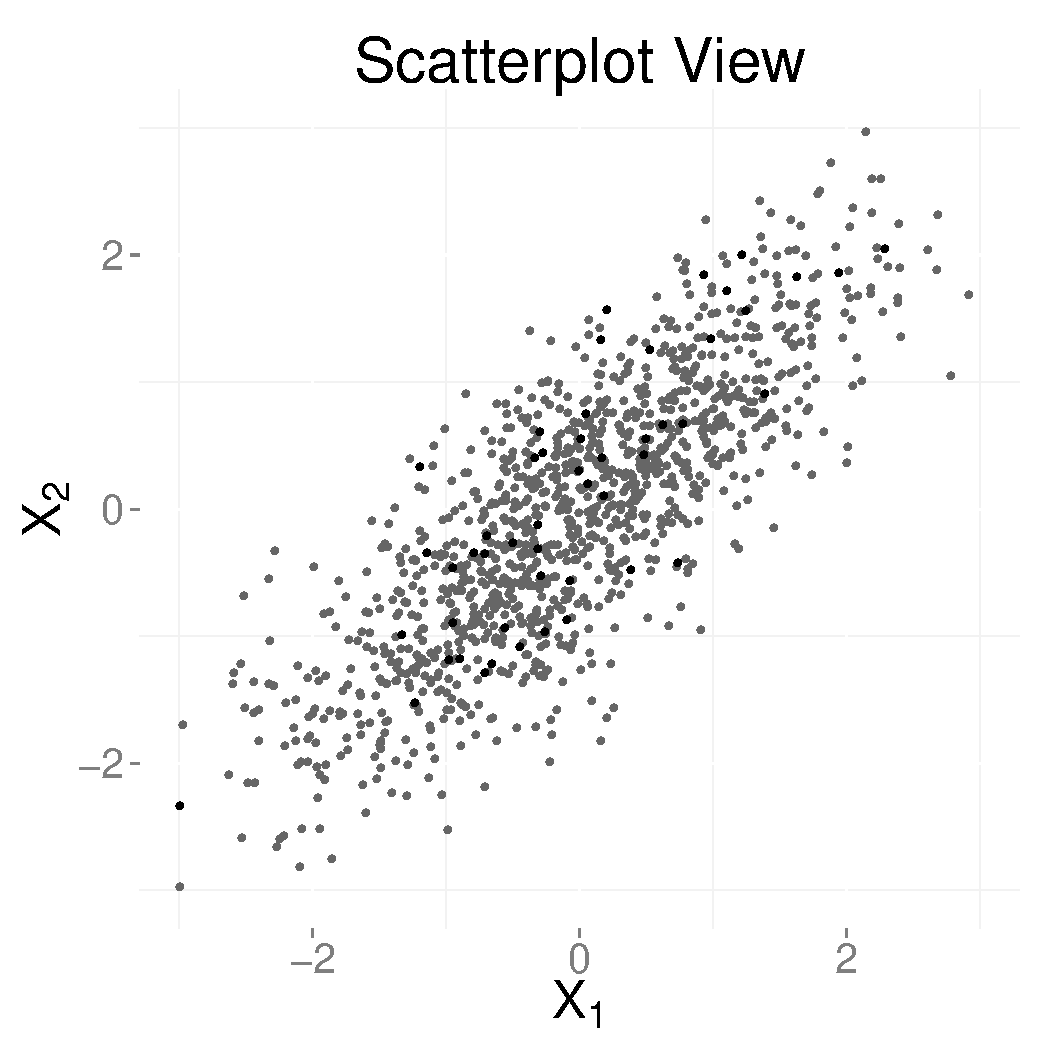
\includegraphics[width=\maxwidth]{figure/scatterplot_function} 

\end{knitrout}

        \tiny
        \begin{itemize} \scriptsize
          \item Highly correlated $\rightarrow$ \textbf{close to diagonal}
          \item Works well for two variables
        \end{itemize}
      \end{column}
      \begin{column}{0.12\linewidth}
\begin{knitrout}
\definecolor{shadecolor}{rgb}{0.969, 0.969, 0.969}\color{fgcolor}
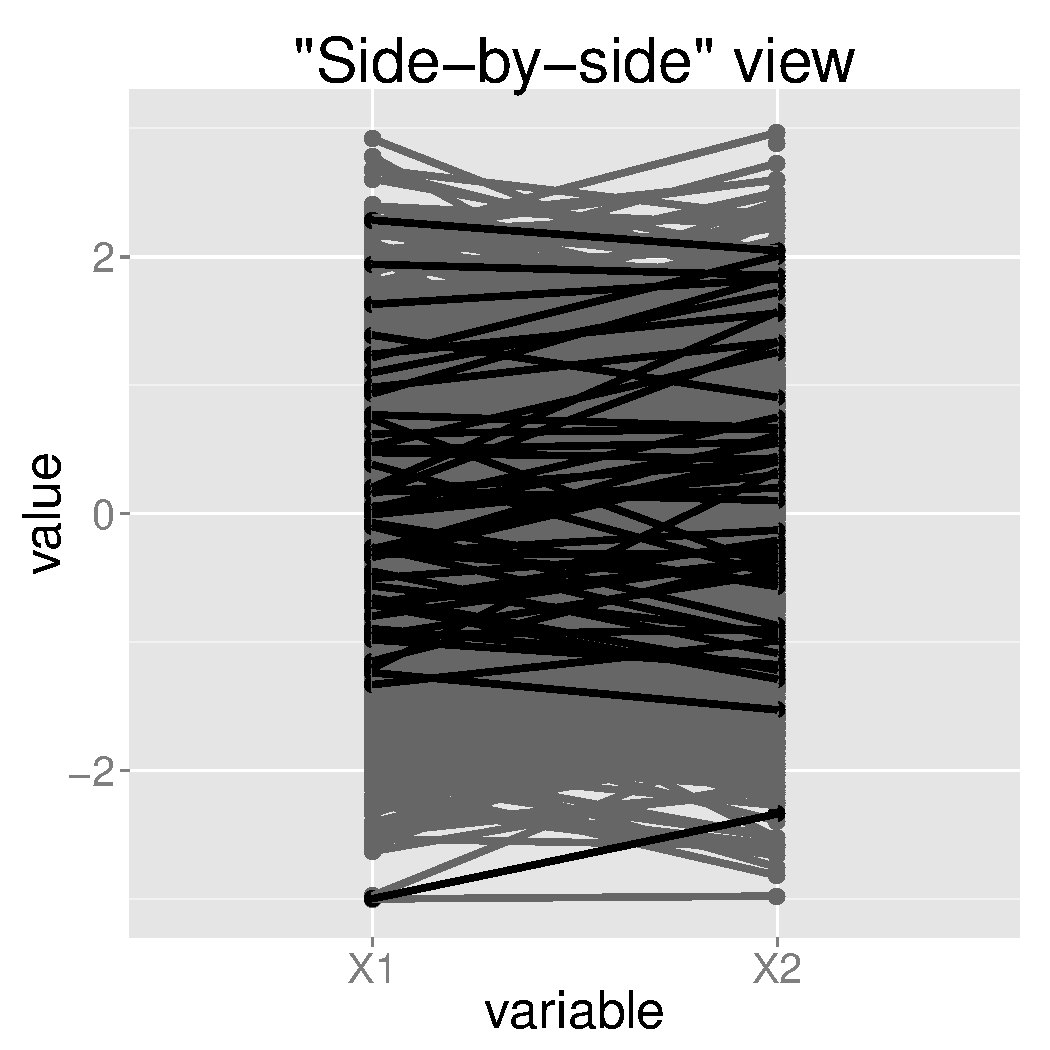
\includegraphics[width=\maxwidth]{figure/side_by_side} 

\end{knitrout}

        \begin{itemize} \scriptsize
          \item Highly correlated $\rightarrow$ \textbf{horizontal lines}
          \item Works well for more variables...
        \end{itemize}
      \end{column}
      \begin{column}{0.12\linewidth}
\begin{knitrout}
\definecolor{shadecolor}{rgb}{0.969, 0.969, 0.969}\color{fgcolor}
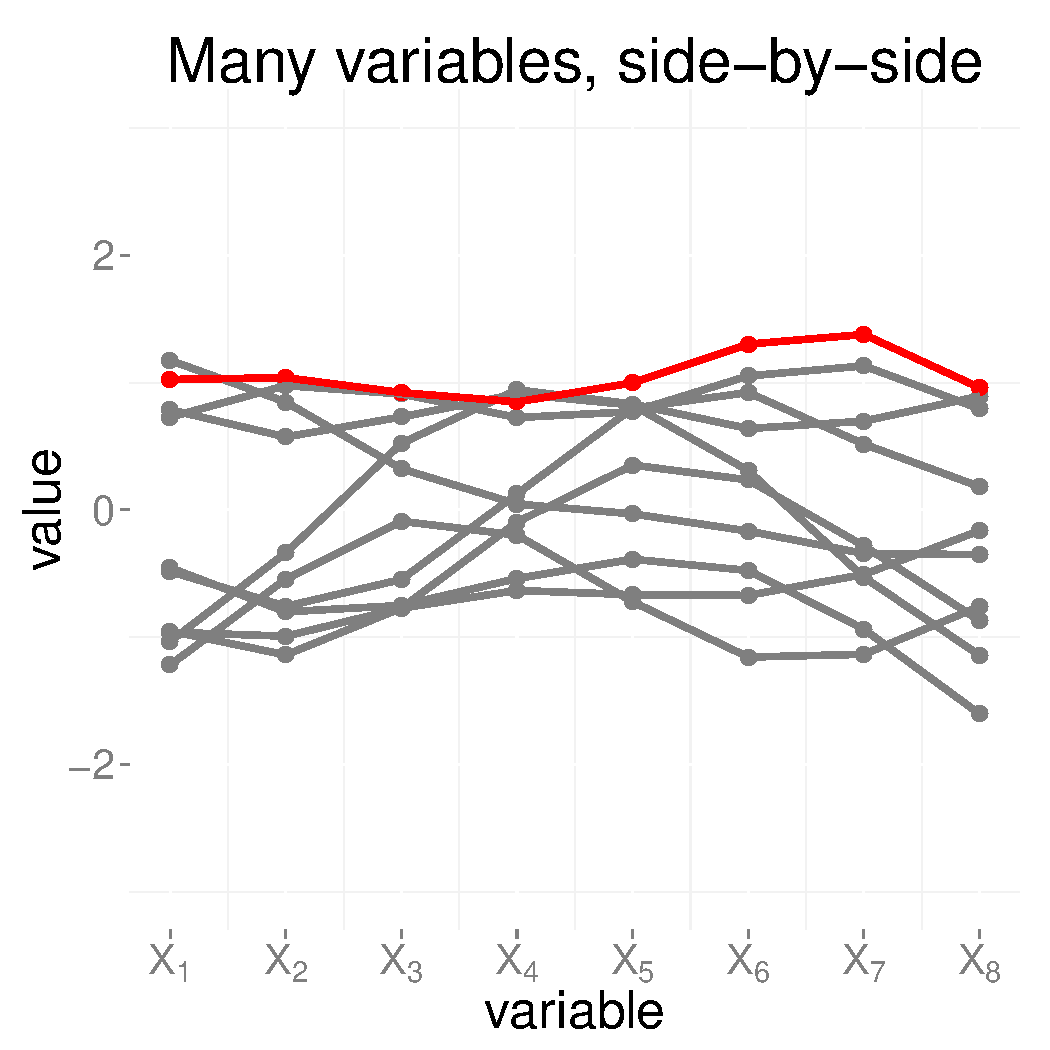
\includegraphics[width=\maxwidth]{figure/many_side_by_side} 

\end{knitrout}

        \begin{itemize} \scriptsize
          \item Variables indexed by \textit{position}
        \end{itemize}
      \end{column}
      \begin{column}{0.12\linewidth}
\begin{knitrout}
\definecolor{shadecolor}{rgb}{0.969, 0.969, 0.969}\color{fgcolor}
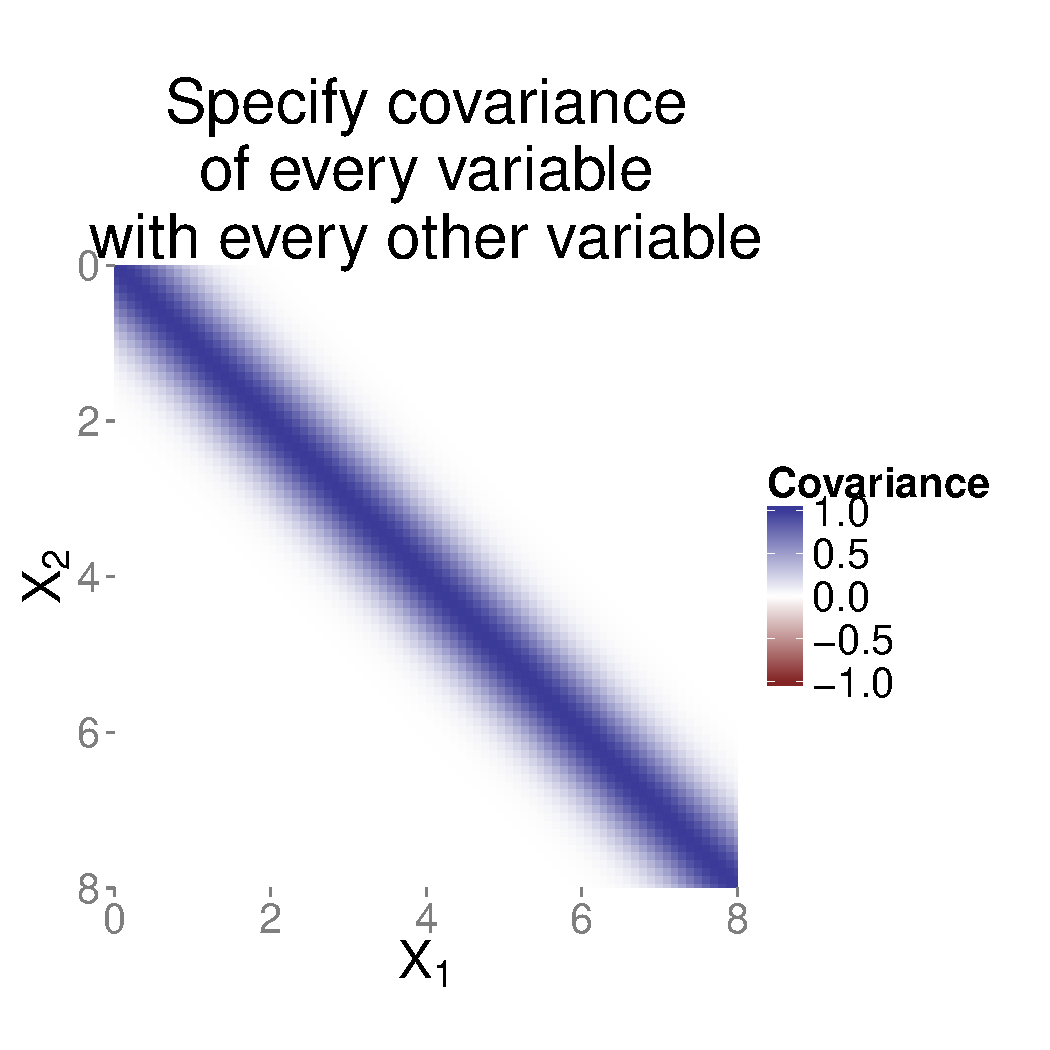
\includegraphics[width=\maxwidth]{figure/covariance_matrix} 

\end{knitrout}

      \end{column}
      \begin{column}{0.28\linewidth}
        \centering
        Get \textit{continuous} random function
        from \textit{I.I.D.} normal draws:
        \vspace{0.4em}
\begin{knitrout}
\definecolor{shadecolor}{rgb}{0.969, 0.969, 0.969}\color{fgcolor}
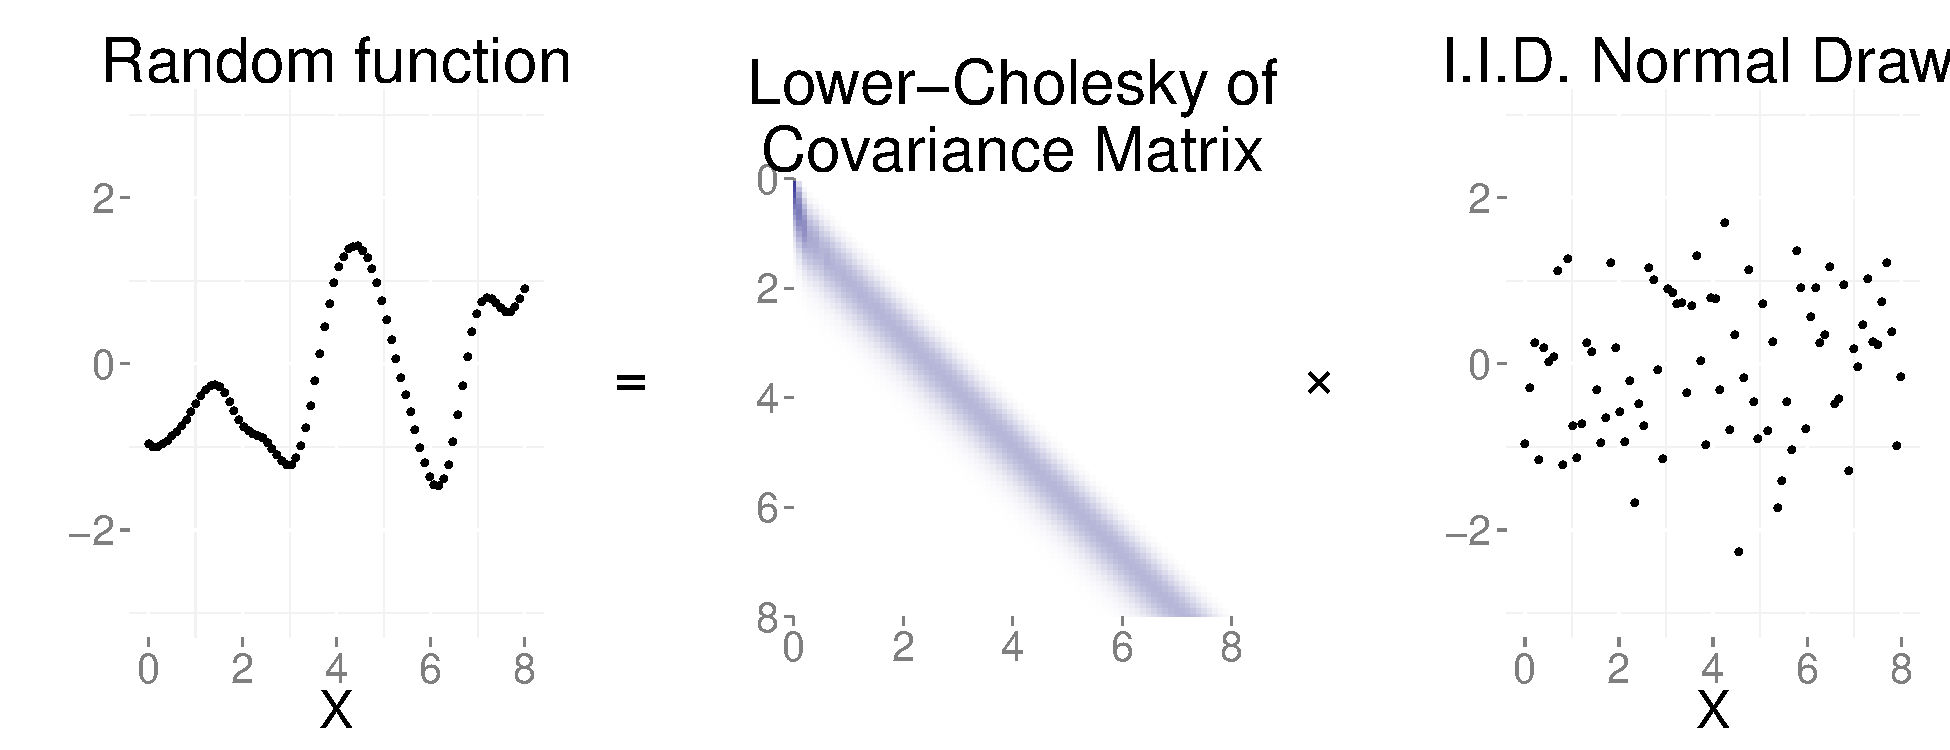
\includegraphics[width=\maxwidth]{figure/random_function_draw} 

\end{knitrout}

      \end{column}
    \end{columns}
  \end{block}
\end{frame}
\end{document}
